\documentclass[a4paper]{article}
\usepackage{lipsum}
\usepackage{url}
\usepackage{graphicx}
\usepackage{listings}
\lstset{language=Python}
\usepackage[margin=2cm]{geometry}
\usepackage{indentfirst}
\usepackage{xcolor}
\usepackage{lmodern}
\usepackage{enumitem}
\usepackage{multicol}
\renewcommand{\familydefault}{\sfdefault}
\graphicspath{ {images/} }

\begin{document}

% TODO: Anything else needed for titlepage
% TODO: Adjust the spacing between bullet point sections
\begin{titlepage}
	\newcommand{\HRule}{\rule{\linewidth}{0.5mm}}
	\center{}

    %Headings
	\LARGE{University of Nottingham}\\[1.5cm]
	\Large{Computer Science with Artificial Intelligence MSci}\\[0.5cm]
	\large{G54IRP/COMP4027 --- Individual Research Project}\\[0.5cm]

    %Title
	\HRule{}\\[0.4cm]
	{\huge\bfseries AI for General Video Game Playing}\\[0.4cm]
	\HRule{}\\[1.5cm]

    %Authors
	\begin{minipage}{0.4\textwidth}
		\begin{flushleft}
			\large
			\textit{Author}\\
			Benjamin Charlton\\
            psybc3@nottingham.ac.uk\\
            4262648
		\end{flushleft}
	\end{minipage}
    \begin{minipage}{0.4\textwidth}
		\begin{flushright}
			\large
			\textit{Supervisor}\\
			Dr.\@ Ender \"Ozcan\\
            Ender.Ozcan@nottingham.ac.uk
		\end{flushright}
	\end{minipage}

    %Date
	\vfill\vfill\vfill
	{\large7\textsuperscript{th} December 2017}
	\vfill

\end{titlepage}

%Contents Page
\pagenumbering{roman}
\tableofcontents
\pagebreak

\pagenumbering{arabic}
\section{Introduction}
\subsection{Introduction}
Game playing has often been used in Artificial Intelligence (AI) research to help push the field forward, developing new techniques to tackle harder and harder problems.
Many of these AI techniques developed have since been applied to further applications proving that this field of study is not just producing novel solutions.
\par
Game Playing is a good testbed for AI techniques due to the many properties of games.
Some of the following reasons show why games make good AI problems:
\begin{itemize}[noitemsep,nolistsep]
    \item Clear win states leading to easy objective evaluation
    \item Limited actions creating fewer output options
    \item Well defined documentation allowing for precise and simple simulations
    \item Testing against different game types as defined in Game theory, such as imperfect information, stochastic outcomes, asymmetric gameplay etc.
    \item Ability to test and rank AIs against human players
\end{itemize}
\par
Artificial Intelligence has been a key component for video games as designers have tried to create compelling single player experiences.
Often AI in video games aren't highly complex often being simple agents optimised for making the player experience fun rather than optimising to win.
For this reason in game AI is often not comparable to academic AI research.
\par
General AI, the ability to create an AI that is deemed generally intelligent that it can complete a wide variety of tasks in many fields, is the ``holy grail'' of the AI field.
Often this level of intelligence is compared to humans, or other animals, as they are good at adapting their knowledge to unseen problems.
Many tests have been thought up to test how to compare the general intelligence of AIs such as the Turing test, Coffee Test or Robot College Student test\cite{AGITests}.
\par
Another strong case for the development of game playing AI is the simplicity of the problem description.
It is a simple problem to define and for the general public to understand what is being achieved, while also being an interesting idea or news item.
This gives the potential for these developments to become news worthy stories and hopefully motivate young people to pursue a career in AI or computer science.

\subsection{Motivation}
The motivation for this project is to see how generalised reinforcement learning techniques can tackle not only video game playing but a general version of this problem.
This showcases the state of the art in both deep reinforcement learning and AI game playing.
\par
Further motivations are more personal, as an individual who would identify as a gamer, seeing a hobby and passion merge with cutting edge AI research is interesting to explore.
The work so far has been enjoyable and intriguing giving the drive and motivation required to do more research and development.
\par
Finally personal development is also a motivating factor.
This project will allow the development of skills in both deep learning and reinforcement learning both gaining a better theoretical understanding of the fields and gaining practical experience implementing these techniques in to functioning systems.
This will come alongside learning how to use robust and powerful frameworks that are used in industry; useful for developing the skills needed for a career in machine learning.

\subsection{Aims and Objectives}
This research project sets out to create and implement a General AI to play video games.
To allow access to a wide variety of video games all with the same interface the project will leverage the GVGAI framework\cite{GVGAI2014}, specifically the Gym variant which allows for learning agents\cite{GVGAIGYM}.
The project will produce several AIs trained using different reinforcement learning techniques as well as producing a research paper comparing the performance of the resulting trained agents.
The objectives of this project are as follows:
\begin{description}
    \setlength{\parskip}{0pt}
    \item [Background Research]
    Perform research into the current state of AI game playing, general AIs, and current well performing solutions to the GVGAI competition.
    The result of this background study will be used to direct the rest of the project and determine a suitable method to tackle the problem with.

    \item [Train multiple General AIs]
    Leveraging the powerful OpenAI Baselines library\cite{baselines}, multiple agent AIs can be trained on various games within the GVGAI Gym framework.
    The reinforcement learning techniques used will come from the selection that the baselines library has to offer, selecting algorithms that have shown promise in related works.

    \item [Evaluation and Analysis of Solutions]
    Compare and analyse the performance of the solutions against each other, previous entries to the GVGAI competition (both learning and planning tracks) and potentially against human players.
    If the solution performs well there may be the ability to test them in unseen environments, such as Video Games that aren't shown in the training sets.
\end{description}
The aims and objectives have changed slightly from the project proposal as implementing a single reinforcement learning algorithm for training didn't seem necessary.
Also although the initial study introducing the GVGAI Gym framework appears to give a baseline evaluation of general AI performance, it trains a separate agent for each of the results allowing for this kind of baseline study to give strong preliminary results to reinforcement learning performance in general video game playing.

\pagebreak
\section{Related Work}
\subsection{AI and Game Playing}
\subsubsection{Early Artificial Intelligence}
The history of AI game playing begins near the start of artificial intelligence as a field, in the 1950s.
Strachey created a draughts player for one of the first general computing machines (Manchester Ferranti Mark I) which by  1952 could ``play a complete game of draughts at a reasonable speed''\cite{BreifHistoryComputing}.
Prinz wrote a simplified chess player for the Manchester Machine as well which could solve the mate-in-two problem.
This meant that if there was a checkmate solution in 2 turns it could successfully find it\cite{BreifHistoryComputing}.
Prinz simply used an exhaustive search technique to find the correct moves, and even though computing power was limited at the time it was clear that this wouldn't scale to full games.
This lead to Turning starting to program `Turbochamp' a chess program that would be able to play a full game of chess using heuristics\cite{BreifHistoryComputing}
\par
These simple games were made before the term artificial intelligence was being used even in an academic setting showing how natural AI and game playing go together.

\subsubsection{Deep Blue --- Chess}
Chess was an early and significant example in the history of AI game playing.
In 1997 IBM managed to beat the reigning world champion, Garry Kasparov, using their custom developed machine, Deep Blue\cite{deepBlue}.
This was significant as, at the time, creating a winning chess AI was seen to be the next big milestone at the time in AI\@.
\par
To achieve this Deep Blue used a combination of techniques with the main underlying AI technique being a search method.
As Chess is a deterministic game and both players have complete information of the board state it was possible for Deep Blue to generate future board states.
With this forward model its possible to generate a search tree of possible moves and their resulting game states
The tree was efficiently generated by a combination of a massively parallel architecture over 30 nodes and the fact that each node has special purpose chess chips, generating around 6--8 moves ahead on average.
Alpha-beta pruning was used in a MinMax algorithm to help efficiently search the tree while using the custom hardware to evaluate each node quickly.
\par
IBM had proven that search methods could achieve strong results against human opponents but this was mostly due to brute force computing power and a heavy reliance on expert knowledge.
The expert knowledge came from other grandmasters and was used in the form of an opening/closing move database and the special purpose hardware to evaluate board states.
While higher computing power will always benefit AI techniques, later techniques have been developed to reduce the need of expert knowledge and to make more efficient use of hardware available.

\subsubsection{AlphaGo --- Go}
Although Deep Blue had proven that AI systems could beat an expert in games, the methods used wouldn't scale to more complex games such as Go, new methods would be needed to tackle more complex games and to further the field of AI\@.
Go was set as the next milestone in AI game playing by the community as it proved vastly more complex than chess while still having few rules and a simple goal, like chess.
To compare the difficulty between the 2 games, chess uses a 8\(\times \)8 board while Go uses a 19\(\times \)19 board.
What is a better indicator of the AI performance is the branching factor of the games for each move, as this more accurately shows how large the search tree grows for each possible move.
On average, Chess has a branching factor of 35 and Go has a branching factor of 250\cite{BranchingFactor}.
In 2016 DeepMind reached this milestone with AlphaGo claiming its victory against a 9th dan professional Go player, Lee Sedol, in March 2016\cite{alphaGo}.
\par
This achievement was accomplished with a combination of Monte Carlo Tree Search (MCTS) and 2 Deep Neural Networks trained with reinforcement learning, one was a value network to assess the board predicting the winner and the other a policy network to predict which move would be played next by an expert.
By augmenting MCTS with the policy network, the problem of the large branching factor was greatly reduced, the value network made the addition that it was quicker and more accurate at determining who would win than conventional methods and didn't require an ending game state to be reached.
Initially these networks were trained on a large number of human played games as a labeled dataset, after this `boot strapping' phase they were trained through instance of self play.
\par
Between October 2015 and AlphaGo's retirement in May 2017 there were 3 significant versions of the AI system.
AlphaGo Fan was named after its opponent Fan Hui a European 2nd dan professional Go player, where it won 5--0 being the first ever computer to beat a human professional at Go without a handicap.
AlphaGo Lee was named after its opponent Lee Sedol a South Korean 9th dan professional Go player, in this match AlphaGo won 4--1 and was seen as an AI system successfully beating a Go champion at their own game.
AlphaGo Master was the final version of the system and was named after the online account it played on for 60 Games against human opponents, it managed to win all 60 games and was finally revealed to have been a computer system to the Go community.
It finally retired at the Future of Go summit where it played a further few games beating another champion Ke Jie and a human team of 5 Go professionals.
After the summit it was clear that AlphaGo was a champion of the game and as a gift to the Go community they presented a series of 50 games for people to analyse.

\subsubsection{AlphaGo Zero --- Go}
After retiring AlphaGo Deep Mind was already working on a successor that would seek to fix some of the downsides of the AlphaGo system.
They sought to create a system that could play `tabula rasa' (latin for from a blank slate) requiring human expert decisions to learn from as they say that `Expert data sets are often expensive, unreliable or simply unavailable'\cite{alphaGoZero}.
The problem came from the initial supervised learning stage of AlphaGo's development, as it required millions of human expert games with the correct outcomes to initially learn from before it began using reinforcement learning and self play to hone its skills.
\par
There are many issues often associated with using supervised learning, 3 of the main issues were brought up when describing the expense, reliability and the availability of these datasets.
While AlphaGo had proven that there was suitable enough data for learning the game of Go, a motivating factor for the team was showing that this wasn't needed and hopefully find a method that could then later be adapted to other problems with these issues.
Another issue was a notion of a skill ceiling, as such to say that the system can only learn to be as good as the data provided to it an idea that is also seen in human learning where a student can only be as intelligent as their teachers.
This was to say that if a system learnt from human experts then it would only slightly build upon the expert knowledge where as their could potentially be ideas unconsidered by humans that could lead to a stronger system.
AlphaGo had shown evidence of this when it played a so-called `divine move' against Lee Sedol indicating there was more potential for innovation in strategy even in an ancient classic game like Go.
Furthermore by also not having a reliance on human expert knowledge an AI system could be developed to complete task where there is limited or no expert knowledge to help guide it.
\par
AlphaGo Zero differs in 4 key ways to its predecessor AlphaGo:
\begin{itemize}[noitemsep,nolistsep]
    \item It trained by selfplay reinforcement learning exclusively, starting with random play.
    \item It only used the 19\( \times \)19 board with the stone colours as input.
    \item It used a single neural network rather than 2.
    \item A simpler tree search was used not requiring a Monte Carlo rollouts
\end{itemize}
By using this form of selfplay it means that AlphaGo Zero gradually improved after every game, but it also allowed for it to have an equally strong opponent at every step of the learning process.
This results in games which much more can be learnt from as it is hard to learn from a system if you are always winning or losing.
\par
The single neural network was designed to take in the raw current board state and output a prediction value of the chance to win and a vector of move probabilities.
This was compared with the true winner of the game from the self play and the search tree probabilities.
The comparison formed the loss function of the neural network and was updated via gradient descent.
\par
The network is used by the search algorithm by selecting the likely moves to make and searching a few moves forward, using the networks winner prediction to select a strong move to make where it has the greatest chance of winning.
\par
Ultimately when tested against different versions of AlphaGo, AlphaGo Zero won with conclusive results.
Winning 100--0 against AlphaGo Lee and 89--11 against AlphaGo Master.
They also gave a rating to a version of AlphaGo Zero that just used the neural network, selecting the move it thought would have the highest probability of winning without using a tree to look ahead.
This neural network only system didn't out perform any version of AlphaGo but it came about 3\% lower than AlphaGo Fan and was 50\% stronger than any other Go AI tested.
\par
Although AlphaGo Zero was intended to work without any human domain knowledge, some was used to help the training process.
In particular the game of Go is invariant under rotation, reflection and colour transposition allowing for the same board to be used for training multiple times, vastly increasing the amount of training data generated for the neural network.
The MCTS that was used to help train the network (not play) was given perfect knowledge of the rules of Go as well.

\subsubsection{Q-Learning and Arcade Learning Environment}
One of the first studies of not just AI video game playing, but tackling the problem with deep reinforcement learning was by Mnih et Al.\ with the use of Q-Learning to play Atari games.
One remarkable thing for the time was the use of raw input from the screen with no specially crafted features.
Another remarkable feature of this research was that only a single network was used for all of the games, although it was retrained for each game.
Both of these elements show that the structure of the network can be applied to game playing in general and no special features are required on a game by game basis.
\par
The Deep Q-networks (DQN) being presented `gave state-of-the-art results in six of the seven games it was tested on, with no adjustment of the
architecture or hyperparameters'\cite{ALE} and in 3 of the games the agent managed to out perform a human expert.
While the DQN was not trained to perform general play the fact that it uses the same network architecture and no human crafted features implies general performance maybe achievable with the larger modern day networks and quicker training times.

\subsubsection{OpenAI Five --- DotA 2}
While board games have found great success in the AI game playing space, video games haven't seen as much popularity due to complexity of both the games and integrating the AI system and the game together.
\par
An attempt to combine AI and game playing was the OpenAI team in the game DotA 2.
DotA 2 is typically a 5v5 team game with a cast of over 100 characters with multiple abilities and items they can use.
It is played from a top down perspective with each game taking place on the same map every time.
As of the time of writing the have been over 10 million unique players in the last month\cite{DotA2}
\par
To help with the complexity of the problem the initial challenge that was tackled was a simpler version of DotA 2 namely 1v1 matches.
Even though this is a scaled down version of the whole game; Elon Musk, backer of this initiative, said that this is `Vastly more complex than traditional board games like chess \& Go'\cite{OpenAI}.
On top of being scaling down the game the team further limited the games to only be played with a single character for both players so that the bot didn't have to learn several character although most 1v1 DotA tournaments use this rule.
The system was first shown off during the 2017 International, the largest DotA 2 tournament featuring a prize pool of nearly \$25 million (USD), to a live audience of DotA 2 fans.
It played a best of 3 1v1 match against one of the best DotA 2 players in history, Dendi, where the AI convincingly won game 1 and Dendi conceded the second game when he realised he was unable to win.
\par
To achieve this astonishing result against not only Dendi but several other professional DotA 2 players, a LSTM Neural Network was trained using selfplay reinforcement learning.
By using the games API it had access to the game state rather than just using the screen input, although this could be seen as an advantage to the AI no information can be got from the API that wouldn't be available to the player looking at the screen.
This allowed for the AI to very easily take input from the game into its neural network and the output to be a valid actions.
\par
The system has been extended into one know as `OpenAI Five', named after the 5 individual neural networks used to create a 5 player team of DotA 2 AIs\cite{OpenAIFive}.
Each of the 5 neural networks are identical but train to play a different character.
These neural networks trained with no human data like AlphaGo Zero, once again proving that contrary to popular belief this isn't needed to create powerful systems.
Unlike a human team the OpenAI Five didn't have a communication channel between the different AIs but were trained to work together and not maximise their reward at the detriment of the teams.
This is a massive step forward towards playing a full game of DotA 2 but there are still some limitations of the system, such as it can only play the same 5 characters and the opposing team also needs to use the same 5 characters.
Certain mechanics of the game were also not implemented into the neural network structure so they can't be used by either the OpenAI Five or its opponents.
Since the initial report some of these restrictions have been lifted and the OpenAI Five can play and play against 18 characters vs 5 originally.
\par
So far OpenAI Five has been performing well against amateur to semi-professional teams, even going as far as beating a team composed of players in the top 99.95th percentile of DotA 2 players.
During the International 8 in August 2018, OpenAI Five played against a top professional team who trained together with most of the restrictions lifted.
This resulted in a game that most people believed to be much closer to the full DotA 2 game.
Unfortunately OpenAI Five lost these games but the team said `Remarkably, the games were exciting and close'\cite{OpenAIInternational}.
The team behind OpenAI Five, OpenAI, believes that the rule changes weren't why they lost, but they need to move forward reducing the number of scripted logic in the system, removing bugs and letting the system train for longer.

\subsubsection{Conclusions}
Conclusions from previous video game playing AIs shown in this section can be summarised as follows.
\begin{itemize}[noitemsep,nolistsep]
    \item Deep Blue shows that game playing AIs can achieve super human performance, although early techniques required a lot of brute force power, human crafted features and sophisticated expert knowledge.
    \item Alpha Go shows that while planning techniques are still effective, ANNs can be used to provided strong performance in games with large search spaces.
    \item AlphaGo Zero and DQN in ALE show that reinforcement learning can be successfully applied to game playing with zero expert knowledge being hand crafted into the system or human knowledge being used to initially train upon.
    \item DQN in ALE and the raw network of Alpha Go Zero show how pure RL algorithms can give strong performance in game playing where a forward model for planning may not be available.
    \item DQN in ALE shows that raw screen input can give strong performance in game playing while OpenAI Five shows that game state maybe sufficient on its own.
    \item OpenAI Five shows that game playing isn't limited to older and simpler games but current popular titles with complex game states can be trained upon to gain near human expert performance.
\end{itemize}

\subsection{VGDL and GVGAI competition}
Levine et Al.\ set out to create a framework to allow for the use of video game playing to be used to help progress the field of general AI\cite{GVGP}.
A similar more naive version of this already existed at the time but focused on board games.
The idea was that a video game playing framework could be used to create a competition to help incentivise research in the area and allow for methods to be shared by many researchers.
This later evolved into the GVGAI framework and competition.
\par
Schaul created a simple way to describe 2D games in their Video Game Description Language (VGDL)\cite{VGDL}.
This allowed for games to be quickly implemented to give a large set of games and levels to train and test on.
Another advantage of the VGDL has been used to spawn a separate track of the GVGAI competition, where an AI has to design new games and levels.
This could be used to dynamically generate more training levels for games without any human skill being required, or even generating entirely new games to test upon.
\par
The current GVGAI competition runs 5 tracks, 2 dedicated to game generation and 3 to game playing.
In particular there is a single player planning, single player learning and 2 player playing tracks.
While the difference between the single and 2 player tracks shows the differences in single and multi agent systems, the planning and learning track show the difference between 2 major forms of game playing algorithms.
\par
Planning methods have a forward model that can be used to internally look ahead at the outcomes after a series of actions have been performed.
The use of this forward model allows the agent to see into the future and chose an action that will give greater long term results.
For planning methods the agents aren't given a chance to train in the environment before running meaning the agent has no prior knowledge of the game before playing it.
Learning methods focus on allowing the agent to practice playing the game (or some close variation of it such as other levels) during a training phase before tackling the problem.
This is closer to how a human expert gets good at game playing and means that it can be used in games/environments where a forward model is complex or not available.
Learning models seem to be more applicable to real world applications due to the lack of a forward model in most scenarios.
\par
After the 2014 GVGAI competition, the organisers, Perez et Al.\ compiled a comparison paper of the entries and how well they performed\cite{GVGAI2014}.
This report clearly shows that planning agents are strongest but could have been due to the lack of a strong RL interface for the GVGAI framework.
Very few of the entries achieved better results than sample agents, with some entries performing worse than random input.
This shows that despite strong evidence that AI can tackle game playing it struggles when moving towards general game playing.
This opens up the opportunity for further research into how best to take general gameplaying forward. 

\subsection{OpenAI Gym and GVGAI Gym}
\subsubsection{OpenAI Gym}
Recently the GVGAI framework has been made to support the OpenAI Gym framework, allowing for each level of every game to be a compatible gym environment.
OpenAI, the creators of OpenAI Gym state that `OpenAI Gym is a toolkit for reinforcement learning research'\cite{OpenAIGym}.
\par
This tool is helpful as it uses a common interface for all of the learning environments, with the hope that this allows RL algorithms to be developed on one problem but easily tested on many others.
For this projects purpose this feature allows the use of open source implementations of popular RL algorithms which are compatible with gym environments to be applied to the problem while reducing problems from poor implementation.
Another benefit of this tool is the ability to independently compare and verify the results of other research knowing that the problem being tested upon is the same due to sharing of benchmark environments.
\par
At each time step an agent can take some input from the environment and process it to get an action to give perform.
After the action is performed the agent receives some basic information; the updated state, reward for that action, is the problem done (this can be due to passing or failing) and some auxiliary information from the environment (typically information could be the environment name and version).
\subsubsection{GVGAI Gym}
As OpenAI Gym environments have proven to be a useful and popular tool amongst RL research, it would be beneficial to create Gym environments for the GVGAI Learning tracks.
This would bring together the benefits of both the GVGAI framework and the Gym framework, allowing for consistent RL interfaces across over 100 games with multiple levels.
This is what was achieved with the GVGAI Gym framework\cite{GVGAIGYM}.
One of the main hopes of this change was that the learning track (which previously didn't see as many entries as other tracks) would be more popular due to ease of use.
\par
The GVGAI Gym environment incorporates all of the previous GVGAI games into their own Gym environments, with each level of the game being its own environment.
This allows for easy splitting of training and validation data, allowing the choice between training on one level and testing on another or even testing on a few games and validating on others.
The games use the incremental score changes as the reward for each time step, in some games this gives a gradual increase in score as the agent performs well and in others it gives a single binary value at the end state of the game.
The agent can receive a mixture of game state opting for a screenshot of the game and/or a serialised state object for the game.
This allows for multiple deep learning methods to be applied from simple artificial neural networks, to LSTM networks even to state of the art convolutional neural networks.

\subsubsection{GVGAI Gym Initial Results}
Some initial finding were made once the GVGAI framework was converted into Gym environments.
In the study Torrado et al.\ used the OpenAI Baselines\cite{baselines} library due to being designed to learn on gym environments.
3 RL algorithms were tested and compared to the state of the art planning algorithms from previous GVGAI competitions\cite{GVGAIGYM}.
Although it appears that the study involved training of a general agent this wasn't the case as each agent was trained on an individual game.
This study is still helpful in showing that RL algorithms can solve some of the games in the GVGAI framework and that the GVGAI Gym environments allow for easy use of other generalised RL algorithm with strong performance.
\par
It was shown in this study that the GVGAI gym environments on average don't perform as well as planning algorithms.
This could possibly be attributed to the advantage a forward planning model provides or simply because the planning agents were taken from strong agents from past competitions and the RL agents were only simple implementations.
What was shown was that on certain games (ones without a binary reward state on completion) were highly successful when applied to RL methods.
\par
Another comparison that can be made is to RL agents trained in the Arcade Learning Environment as many of the games in the GVGAI framework are based upon simple Atari games, as well as both environments giving the raw screen data as a form of input\cite{ALE}.
Although not directly comparable as the games are different the results suggest that the GVGAI Gym variants perform as well as Arcade Learning Environment counterparts suggesting that this performance maybe extended to other games in the GVGAI Gym framework.
\par
The fact that this study doesn't test the general performance of the baselines library on the GVGAI Gym environments allows for a strong opening for furthering this area of research which is what this project aims to investigate and tackle.

\subsection{Subsection to end all subsections}
\begin{itemize}
    \item Maybe something about the open AI baselines
    \item Depends what technique I would be using but I should look into that
    \item Where does reinforcement learning come into this bad buoy
\end{itemize}

\pagebreak
\section{Progress}
In this section the progress made up until the writing of this report will be discussed alongside any modifications that were made to the work plan, changes to future plans based upon the work so far will be discussed in the next section.
\subsection{Modifications to the Work Plan}
Some tasks have been modified to due to various factors, such as them taking longer than expected or new additions to help make easier progress.
An up to date version of the work plan has been included in the appendix showing an accurate depiction of what tasks were completed over the previous term, with changes highlighted in a bold box.
This can be seen in TODO INSERT SECTION 5.3.1.
Following is a list of modifications that have been made and the reasons behind these changes.
\begin{description}
\setlength{\itemsep}{0pt}
\setlength{\parskip}{0pt}
\item [\large{Documentation}]
\item [D4--Interim Report Outline Sections]
This was pushed back a week to accommodate for the addition of task C5.
\item [D5--Interim Report Related Work]
Extended the writing of the related work section due to the larger amount of research done that was needed to be talked about.
This is due to the project taking a large research focus for the first term than initially expected and compared to previous projects.
\item [D6--Interim Report Draft]
This was pushed back a week to accommodate for the addition of task C5.
\end{description}

\begin{description}
\setlength{\itemsep}{0pt}
\setlength{\parskip}{0pt}
\item [\large{Research}]
\item [R5--Other Related Works]
This was extended from 2 to 4 weeks to accommodate for the addition of task C5 and to allow for more papers to be researched after seeing a wide variety of relevant and informative papers.
\end{description}

\begin{description}
\setlength{\itemsep}{0pt}
\setlength{\parskip}{0pt}
\item [\large{Development}]
\item [S3--Run available previous agents]
As there was no previous agents available using the latest framework, previous agents couldn't be ran in the same framework that the project was being developed in.
Rather than spending time installing a previously used framework it was decided that it would be simpler and more effective to just use the results in the research articles instead of running the agents to compare them.
\item [S5--Develop Keyboard Controller]
While trying to debug some issues with the framework it became clear that it would be easier to test if the GVGAI games could be directly controlled by a user.
For this reason a keyboard controller was made to allow for user controlled games.
\end{description}

\begin{description}
\setlength{\itemsep}{0pt}
\setlength{\parskip}{0pt}
\item [\large{Miscellaneous}]
\item [M4--Plan 2\textsuperscript{nd} Stage of the Project]
This part was brought forward a week to align with the writing of this report.
This allows for this report to contain a plan for the second stage and moving it forward doesn't massively clash with other aspects of the project.
\end{description}

\begin{description}
\setlength{\itemsep}{0pt}
\setlength{\parskip}{0pt}
\item [\large{Other Commitments}]
\item [C5--GameSoc Varsity \& HackNotts]
This was added as 2 large university society events that I was volunteering at were taking place during this time.
This meant that project work was postponed to allow concentration on the successful running of these events
\end{description}

\subsection{Current Achievements}
In this part, any significant progress will be described outlining what was done and how it has helped the project move forwards.

\subsubsection{Learning the GVGAI, OpenAI Gym and GVGAI Gym Frameworks}
A lot of time has been spent learning various frameworks that are used within the GVGAI competition and will be used in this project.
By using these frameworks significant amounts of work that would be required to create games or successfully interface with previous ones has been reduced.
Despite this time has still been spent on learning hope the frameworks operate to use them effectively.
Some of the following achievements put the knowledge gained from learning these frameworks to use in creating useful tools.

\subsubsection{Action Space Analysis}
Due to how recent the GVGAI Gym framework is, some elements of the how the games worked were unclear.
One such element was the action space of the agents which corresponds to the inputs for the games.
To answer any questions, a small script was written to analyse the action space of all the environments.
\par
The following was discovered:
\begin{description}
\setlength{\itemsep}{0pt}
\setlength{\parskip}{0pt}
\item [Total number of actions]
Across all the games the same 6 actions were used, listed below with their typical meanings.
\begin{multicols}{2}
    \begin{itemize}[noitemsep,nolistsep]
        \item ACTION\_NIL --- Make no action
        \item ACTION\_USE --- Interact in game
        \item ACTION\_LEFT --- Move the character left
        \item ACTION\_RIGHT --- Move the character right
        \item ACTION\_DOWN --- Move the character down
        \item ACTION\_UP --- Move the character up
    \end{itemize}
\end{multicols}
\item [Not all games used all actions]
While every game had a ACTION\_NIL action, some games didn't use all of the other actions.
This means that for some games the action space is smaller than others and this would have to be taken into account when making an AI to play all the games, as trying to use an incorrect action could cause unpredictable behaviour in a AI system but will also result in disqualification in the GVGAI competition.
Simple solutions to this problem could be passing an ACTION\_NIL if the AI tries to use an action that isn't available in the current game, or to selected the next best choice of action as given by the AI\@.
\item [The Actions weren't numbered the same]
The action descriptions have been used so far to give an idea of what each action does, the labels are from the old GVGAI framework where these where used as an enum to describe each action.
In a discrete OpenAI Gym environment, which the current GVGAI Gym is, the action space is represented as a set of numbers corresponding to the actions order.
While the actions are always ordered the same way (ACTION\_NIL will always be first and ACTION\_UP last) if an action is not used in that game and therefore not present it will mess up the numbering.
This means care needs to be taken in games that don't use all the actions so that the correct action is given to the environment.
\end{description}

\subsubsection{Keyboard Controller}
It became apparent that a way for a human to interact with the various environments would prove useful for development and debugging.
The majority of the code for this was reused from the OpenAI Gym keyboard controller\cite{OpenAIGym}, which can be found in their GitHub repository.
\par
The modifications made allowed for relevant logging to the console, better controls, displaying the controls to the user at the start, and setting a game tick rate/ frame rate to be the same as the GVGAI competition.
The WASD keys were bound to movement and use on the J key, this is closer to what typical games would use making it easier to pick up for people used to playing on a keyboard already.
The frame rate is set rather low for games at 25fps but it can be changed in the program, 25fps is used as that is both smooth enough and gives the same decision and reaction time as the AI system will get.
Although this does make it much simpler for any human player to succeed in trickier parts of a game, even making frame perfect timing relatively easy for most humans.
\par
Although originally intended to aid development this tool could be used to compare an AI system against human skill of varying levels.

\subsubsection{Random Agent}
To help understand the framework and to generate a point of comparison, a simple random agent was made.
It works by knowing the the possible actions across all games and choosing one at random, if that action isn't in the list of actions in the game currently being played it will then reselect an action.
This is a simple solution to get around the fact that not all actions are used in all games.
It samples all actions uniformly with no bias to a particular action.
\par
The random agent is wrapped in a program that allows it to be ran in any of the environments.
There are also settings to allow the choice of rendering the game screen to the user so the agent actions can easily be shown, as well as a setting to modify the number of game ticks that the game will be ran for.

\subsubsection{Testing Agent in multiple Environments}
Another help tooler created was one that could run a given agent in multiple of the environments to test how well it performs in the environments.
It is currently set up to run the random agent in all of the environments (bar a few that have been crashing).
It also runs the agent in each environment a few times so that random variation (in the game or agent) can be accounted for.
\par
As there are many environments to run the agent in, this tool makes effective use of multiprocessing allowing a significant speed up in the generating of data.
For each run in an environment the following data is collected:
\begin{multicols}{2}
    \begin{itemize}[noitemsep,nolistsep]
        \item Game --- The game being played
        \item Level --- The level of the game
        \item Version --- The game version
        \item Score --- The final score at the game end
        \item Winner --- Wether the agent won
        \item Game Tick --- The game tick when the game ended
    \end{itemize}
\end{multicols}
These results are stored as a json object and parsed together with all the other results to create a list of all of the results.
As the list is in a json format it can be easily analysed at a later date, or combined with other runs to create a larger dataset.
\par
\begin{itemize}
    \item Do I analyse and put the random agent results in here?
\end{itemize}
\par
This tool will become incredibly useful when testing an agents performance across a variety of games due to its quick running time.
It is also simple to test multiple agents using this tool so that they can be compared to each other.
As the tool returns the raw data it can be analysed in whatever way suits the current scenario, such as even though the random agent has been run in all of the environments we can easily compare it to another agent in a handful of those environments by simply selecting the correct data points from the random agent results for comparison.

\subsection{Reflections on Current Progress}
On the whole the work plan has been stuck to, allowing for easy knowledge of where the project is up to at any time and clear progress to be made.
The minor changes to the work plan have on the whole been made to aid with management of large tasks and other commitments.
Although a few tasks were delayed the major milestones have been stuck to so far, namely finishing of development tasks and writing the interim report.
\par
A personal issue with progress was the lack of deliverables with the major research section of the project.
This section took up over 50\% of the time spent on the project so far.
This time was spent by self guided study, finding and reading relevant works to the project.
With the lack of deliverables it was hard to judge if enough research had been completed, or if a wide enough scope was researched.
Another issue with the research was time spent researching and understanding older frameworks which bare little to no relevance on the project moving forward.
Spending hours researching a topic to only realise it is not what you thought it was on initially led to some frustration.
\par
To aid with project management and accountability meetings have taken place, with a regular slot set aside to allow for agile meetings.
These have often discussed upcoming tasks in relation to the work plan and what work has taken place.
For each meeting a short set of minutes was created and emailed to attendees, allowing for all parties to know what was discussed and what was to happen before the next meeting.
All of the minutes can be found in the appendix, section TODO INSERT SECTION 5.2.

\pagebreak
\section{Next Steps}
This section will outline the next steps in the project as directed by the research done into what methods are effective.
All of these steps are also outlined in the work plan and can be seen in the appendix section TODO INSERT SECTION 5.3.2.
\subsection{Modifications to existing code}
The current random agent and tool to run an agent in multiple environments doesn't use a preexisting class for agents.
This is due to the fact an agent class wasn't given in the GVGAI Gym framework when these elements were developed.
As these definitions exist all agents moving forwards can properly inherit from the agent class.
\par
To make use of this agent class, the agent and running script need to be updated to use them.
This will help with compatibility and reusability of code in the project.
It should also allow others to use the agents easily or, if any agents are released during the project, those agents to be compared with each other.
\par
This is set as task S6 --- Refactor to match Agent Structure in the work plan.

\subsection{Breaking down Tasks R6 and S4}
Tasks R6 and S4 for initially placeholders for the research and development of the final solution respectively.
This was due to prior research needing to take place before these tasks could be accurately broken down into subtask.
With the research from this section of the project completed it is possible to break down these tasks into appropriate sub tasks.
\par
The as stated in the aims and objectives (section TODO INSERT SECTION 1.4.) the project will aim to use several of the reinforcement learning algorithms in the OpenAI Baselines framework to general video game playing.
This will involve selecting which RL algorithms to use, integrating the gym environments to run on the selected RL algorithms, and effectively setting the hyper-parameters for selected RL algorithms.
It will also take a while to train all and validate all of these agents so that has also been accounted for in the work plan.
\par
Following is a list of how the tasks have been broken down and what each sub task entails.
\begin{description}
\setlength{\itemsep}{0pt}
\setlength{\parskip}{0pt}
\item [\large{Research}]
\item [R6.1--Baselines Basic Research]
This task is to research the OpenAI Baselines framework to help understand how it all works.
It will be done alongside S4.2 to help gain a practical understanding.
\item [R6.2--Research effective RL Algorithms]
During this task research into the reinforcement learning algorithms used in the related work examples will be used to guide which RL algorithms to focus on in the development of the final solutions.
Other details such as hyper-parameters will also be researched in this task.
\item [R6.3--Select Final Comparison Methodology]
Based upon the initial performance of the baselines, a methodology for comparing the resulting agents together.
This will involve deciding which games/levels to give access during training and validation.
\item [R6.4--Analyse the Results]
Once all the agents have trained and been tested, this task will aim to analyse the results to glean some interesting information.
\end{description}

\begin{description}
\setlength{\itemsep}{0pt}
\setlength{\parskip}{0pt}
\item [\large{Development}]
\item [S4.1--Install OpenAI Baselines]
Simple task to get all of the required parts of the framework installed and working properly.
It will also involve properly integrating it with the code base's virtual environment to allow easy moving to another system.
\item [S4.2--Integrate Baselines on 1 Game]
This task aims to help gain an understanding of the OpenAI Baselines framework by getting a single game to train through it.
This should help gain the base understanding of the framework while testing how to run it effectively on powerful hardware such as a GPU\@.
To help check if it has been successfully implement comparisons to the initial GVGAI Gym paper can be made as it explored this idea\cite{GVGAIGYM}.
\item [S4.3--Integrate Logging via TensorBoard]
TensorBoard is a powerful tool to help watch the training of various RL algorithms on neural networks.
It should be possible to use this to help keep track of how well the agent is performing over the learning process.
\item [S4.4--Baselines on Multiple Games]
Alongside task R6.2, the selected RL algorithms will be integrated to train on multiple games.
Once it can train on multiple games it should be fairly trivial to limit it to only a select few levels of the games if that is required.
\item [S4.5--Train Agents for Comparison]
Once the final comparison methods have been chosen in task R6.3, they can be implemented and ran so that the agents can train.
This could take a while to successfully complete depending on the scope of the agents generality.
This task may also overrun into the writing of the final paper but as most tasks in the writing process can be done without the final results this shouldn't be an issue.
\item [S4.6--Validate the Trained Agents]
Once the agents have been trained this task can evaluate the agents performance across the relevant games and levels to see how well it performs.
\end{description}

\pagebreak
\section{Appendix}
%Bibliography
\subsection{References}
\renewcommand\refname{\vspace{-1cm}}
\bibliography{InterimReport}
\bibliographystyle{plain}

\subsection{Meeting Minutes}
\subparagraph{25th October}
Recap of the submitted project proposal. \\
Discussed the lack of proposed methodology in the proposal, due to competition framework not being researched fully. Agreed to have a stronger idea with the interim report. \\
Overview for the next stage of the work plan, researching and understanding the GVGAI Framework --- specifically looking into the Learning track. \\
Agreed to meet on Wednesdays 2--2:30 as required.

\subparagraph{14th November}
Progress report. \\
Created a keyboard controller interface to play games. \\
Created a random agent and a way to run this on all 100 games to provide a comparison point. \\
Unable to run previous agents as none are available from the new framework although some may be available soon. \\
Could run a baseline learning implementation as discussed although this will take some time to implement and run. \\
Current research is going well ready to start work on the interim report specifically background research. \\
Will look into overleaf for sharing of the interim report drafts.

\pagebreak
\subsection{Work Plan}
Some rows have been removed when they aren't showing a task in the time frame shown.
\subsubsection{24\textsuperscript{th} September --- 7\textsuperscript{th} December}
\begin{center}
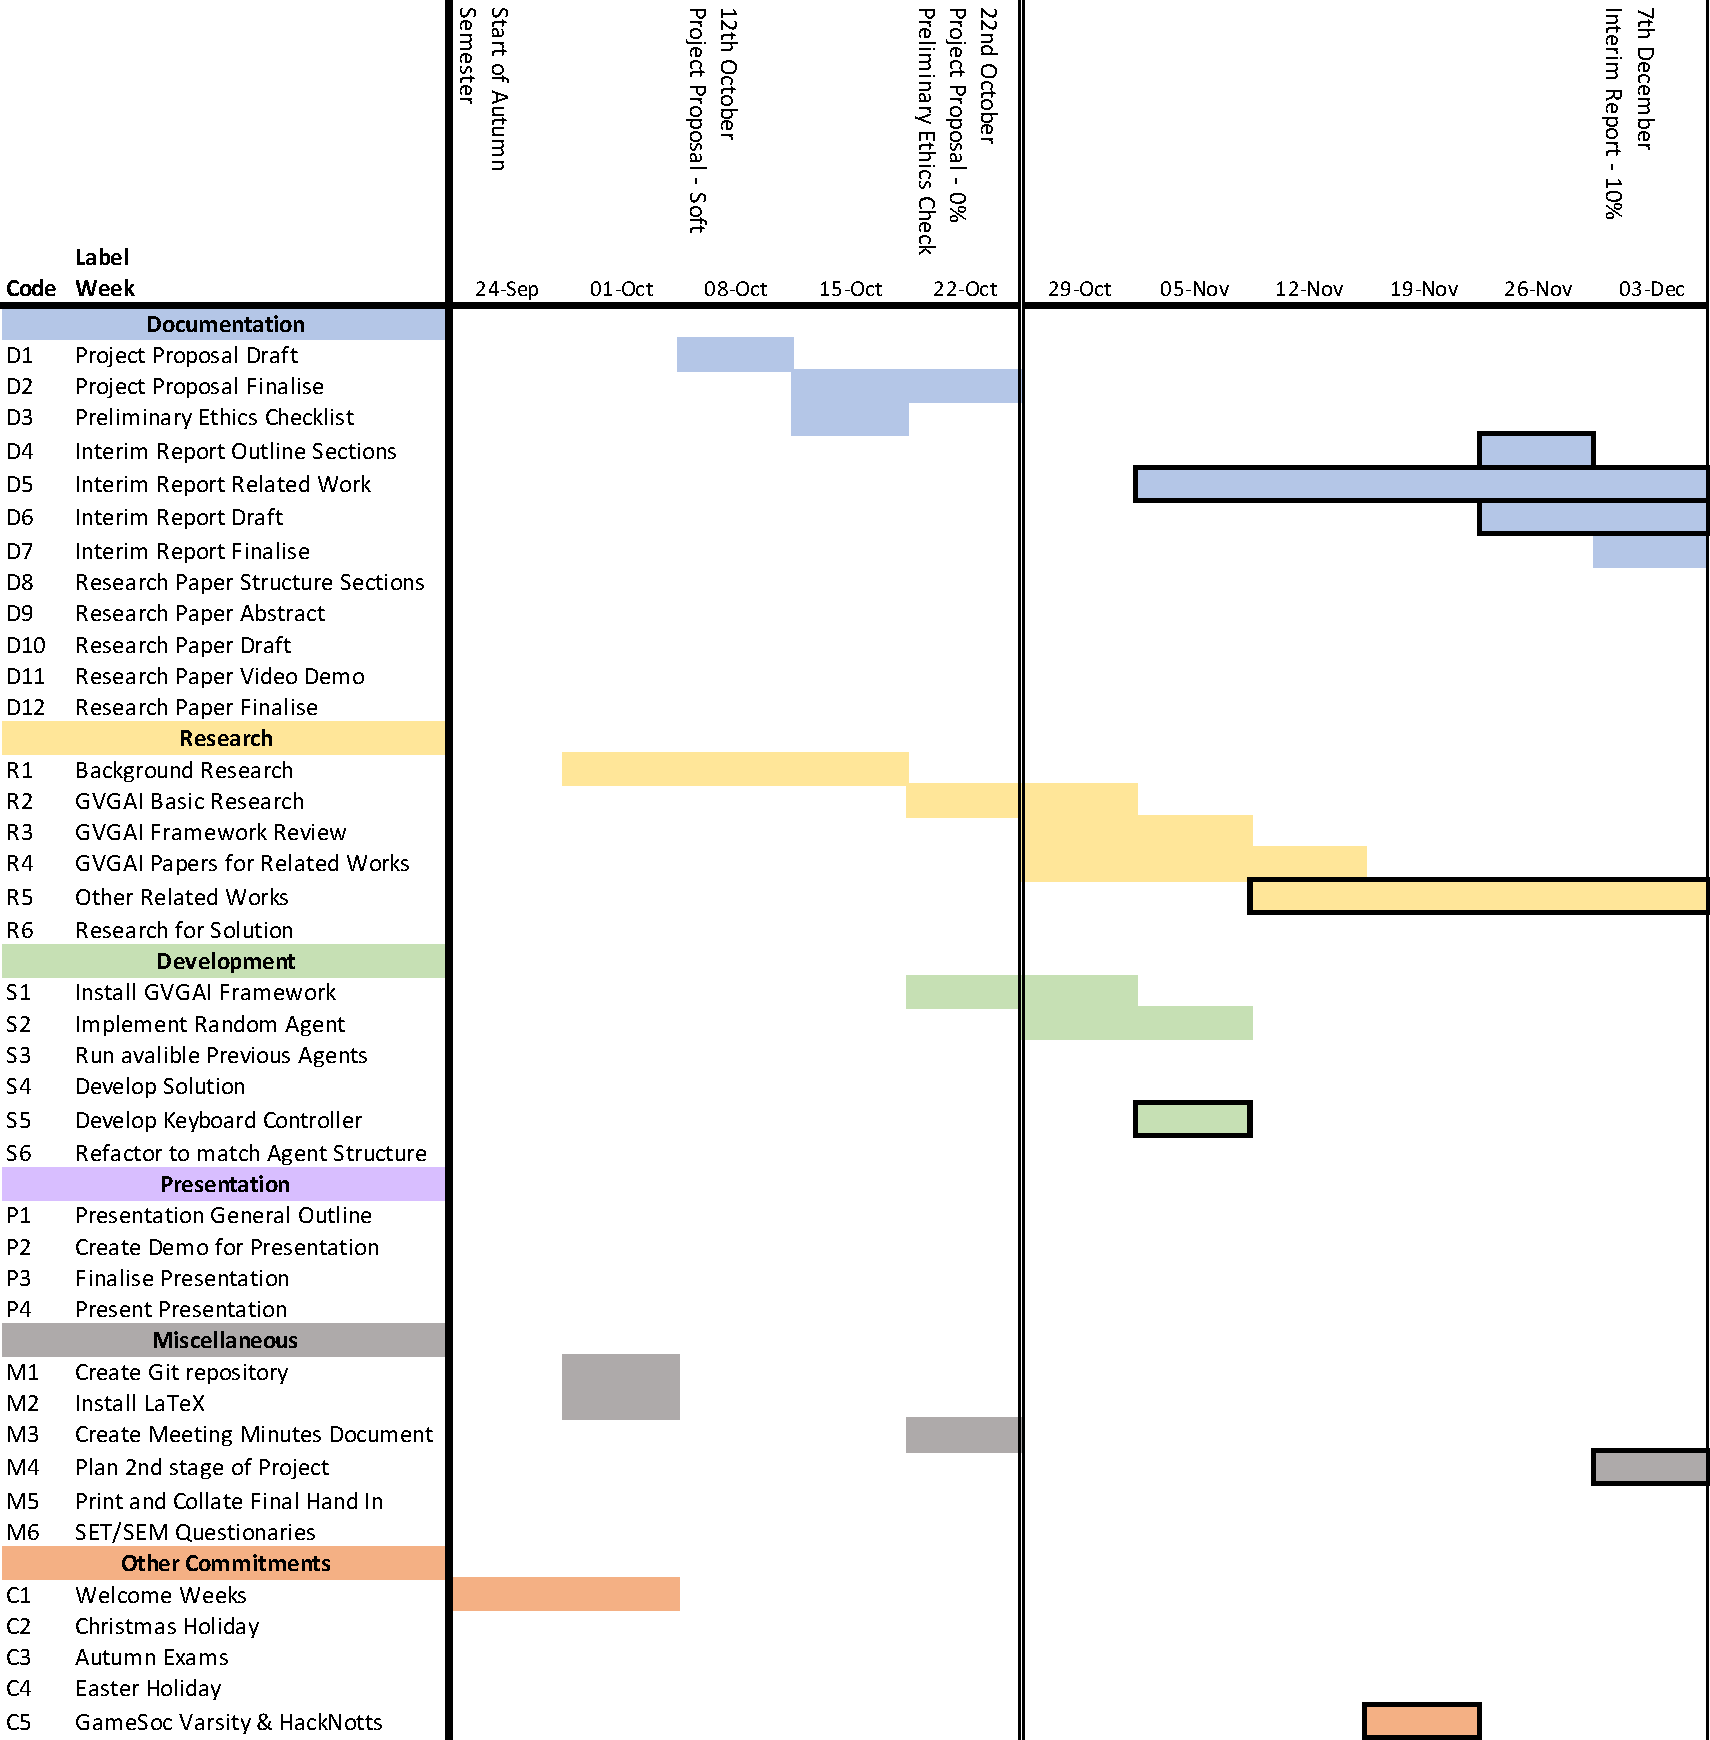
\includegraphics[width=17cm]{workPlan-7Dec.pdf} %17cm is 21cm of A4 width - (2cm * 2) margins
\end{center}
\subsubsection{7\textsuperscript{th} September --- 17\textsuperscript{th} May}
\begin{center}
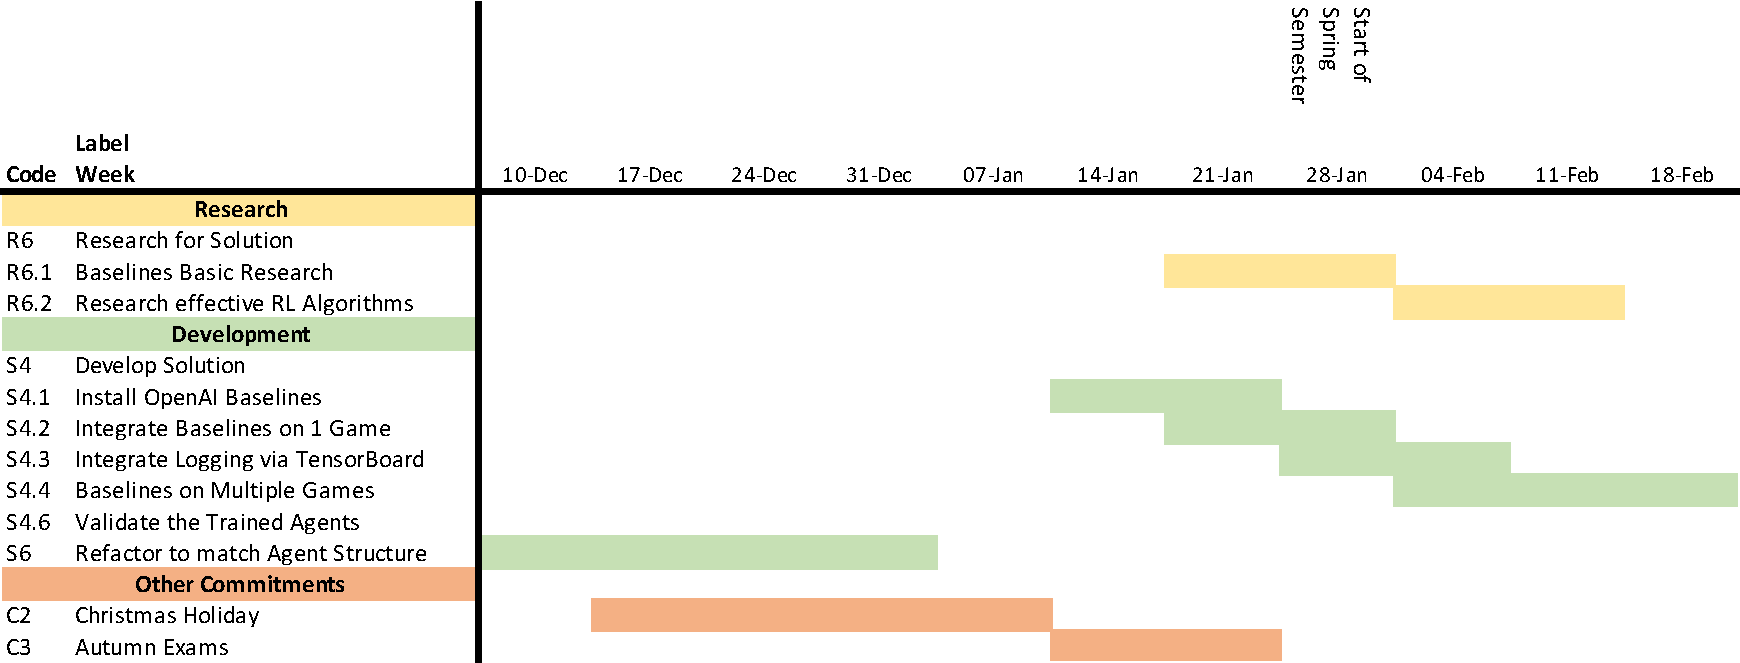
\includegraphics[width=17cm]{workPlan-18Feb.pdf} %17cm is 21cm of A4 width - (2cm * 2) margins
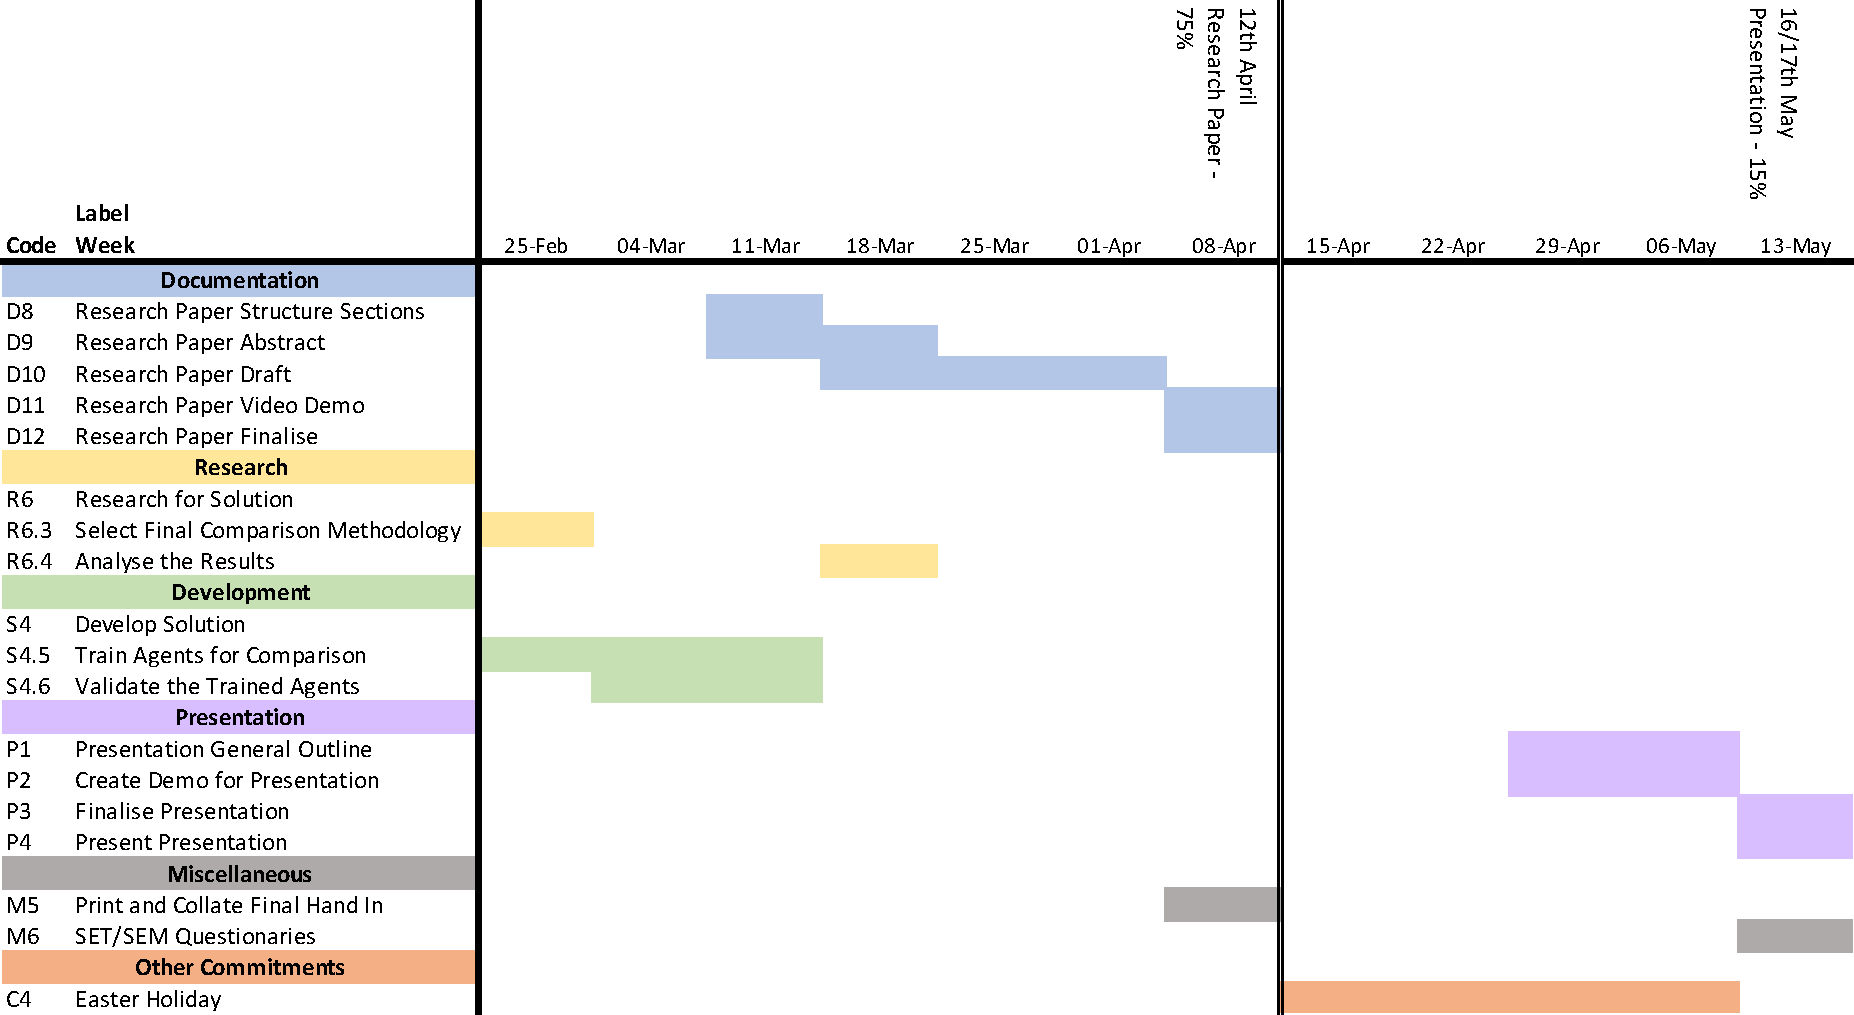
\includegraphics[width=17cm]{workPlan-17May.pdf} %17cm is 21cm of A4 width - (2cm * 2) margins

\end{center}


\end{document}
